\documentclass[12pt,a4paper,reqno]{amsart}

% language
\usepackage[greek,english]{babel}
\usepackage[utf8]{inputenc}
\usepackage{alphabeta}

% change default names to greek
\addto\captionsenglish{
    \renewcommand{\contentsname}{Περιεχόμενα}
    \renewcommand{\refname}{Βιβλιογραφία}
    \renewcommand{\datename}{Ημερομηνία:}
    \renewcommand{\urladdrname}{Ιστοσελίδα}
}

% math 
\usepackage{amsmath,amsthm,amssymb,amscd}

% font
\usepackage[cal=euler]{mathalfa}
\usepackage{libertinus-type1}
% \usepackage{txfonts} % for upright greek letters
\usepackage{bm} % for bold symbols
\usepackage{bbm} % for the simply-looking bb symbols

% miscellaneous 
\usepackage{changepage} %for indenting environments
\usepackage{csquotes} % example: \textcquote{}
\usepackage{blkarray}
\setcounter{MaxMatrixCols}{20} % default for pmatrix is 10!!
\usepackage{ytableau}
\usepackage{array} %needed to increase the vertical length in a tabular

% drawing
\usepackage{tikz,tikz-cd}
\usetikzlibrary{shapes.misc, patterns, matrix, calc, intersections,positioning,arrows.meta}
\usepackage{graphics,graphicx}
\usepackage{float} % provides enhanced control and customization options for floating objects such as figures and tables

% colors
\usepackage{xcolor}
\definecolor{darkcandyapplered}{rgb}{0.64, 0.0, 0.0}
\definecolor{midnightblue}{rgb}{0.1, 0.1, 0.44}
\definecolor{mylightblue}{HTML}{336699}
\definecolor{burntorange}{rgb}{0.8, 0.33, 0.0}
\definecolor{iceberg}{rgb}{0.44, 0.65, 0.82}
\definecolor{applegreen}{rgb}{0.55, 0.71, 0.0}
\definecolor{canaryyellow}{rgb}{1.0, 0.94, 0.0}
\definecolor{lightgray}{rgb}{0.83, 0.83, 0.83}

% hrefs
\usepackage{hyperref}
\usepackage[noabbrev,capitalize]{cleveref}
\hypersetup{
    pdftoolbar=true,        
    pdfmenubar=true,        
    pdffitwindow=false,     
    pdfstartview={FitH},  % fits the width of the page to the window
    pdftitle={},
    pdfauthor={},
    pdfsubject={},
    pdfkeywords={},
    pdfnewwindow=true,  % links in new window
    colorlinks=true,  % false: boxed links; true: colored links
    linkcolor=darkcandyapplered,   % color of internal links
    citecolor=midnightblue,  % color of links to bibliography
    urlcolor=cyan,  % color of external links
    linktocpage=true  % changes the links from the section body to the page number
    }

% geometry
\textwidth=16cm 
\textheight=21cm 
\hoffset=-55pt 
\footskip=25pt

% thm envs (you might need to change the path)
\theoremstyle{definition}
\newtheorem{theorem}{Θεώρημα}
\newtheorem{proposition}[theorem]{Πρόταση}
\newtheorem{lemma}[theorem]{Λήμμα}
\newtheorem{corollary}[theorem]{Πόρισμα}
\newtheorem{conjecture}[theorem]{Εικασία}
\newtheorem{problem}[theorem]{Πρόβλημα}
\newtheorem*{claim}{Ισχυρισμός}
\newtheorem{observation}[theorem]{Παρατήρηση}
\newtheorem{definition}[theorem]{Ορισμός}
\newtheorem{question}[theorem]{Ερώτημα}
\newtheorem*{questions}{Ερωτήματα}
\newtheorem*{que}{Ερώτημα}
\newtheorem{example}[theorem]{Παράδειγμα}
\newtheorem{exercise}{Άσκηση}

\theoremstyle{remark}
\newtheorem*{remark}{Παρατήρηση}

% fixes the correct numbering of environments
\numberwithin{theorem}{section}
\numberwithin{exercise}{section}
\numberwithin{equation}{section}

% math ops 
% fields
\newcommand{\NN}{\mathbbmss{N}} 
\newcommand{\ZZ}{\mathbbmss{Z}} 
\newcommand{\QQ}{\mathbbmss{Q}} 
\newcommand{\RR}{\mathbbmss{R}} 
\newcommand{\CC}{\mathbbmss{C}} 
\newcommand{\KK}{\mathbbmss{K}} 
\newcommand{\FF}{\mathbbmss{F}} 
\newcommand{\HH}{\mathbbmss{H}} 

% symmetric group
\newcommand{\fS}{\mathfrak{S}}  

% calligraphic 
\newcommand{\aA}{\mathcal{A}} 
\newcommand{\bB}{\mathcal{B}}
\newcommand{\cC}{\mathcal{C}}
\newcommand{\dD}{\mathcal{D}}
\newcommand{\eE}{\mathcal{E}}
\newcommand{\fF}{\mathcal{F}}
\newcommand{\hH}{\mathcal{H}}
\newcommand{\iI}{\mathcal{I}}
\newcommand{\lL}{\mathcal{L}}
\newcommand{\oO}{\mathcal{O}}
\newcommand{\pP}{\mathcal{P}}
\newcommand{\sS}{\mathcal{S}}
\newcommand{\mM}{\mathcal{M}}
\newcommand{\uU}{\mathcal{U}}

% bold
\newcommand{\bfa}{\mathbf{a}}
\newcommand{\bfe}{\mathbf{e}}
\newcommand{\bfF}{\pmb{F}}
\newcommand{\bfR}{\pmb{R}}
\newcommand{\bfv}{\mathbf{v}}
%\newcommand{\bfx}{\bm{x}}
%\newcommand{\bfx}{\mathbf{x}} 
\newcommand{\bfx}{\pmb{x}}
\newcommand{\bfX}{\pmb{X}}
\newcommand{\bfy}{\pmb{y}}
\newcommand{\bfz}{\pmb{z}}

% roman
\newcommand{\rmA}{\mathrm{A}}
\newcommand{\rmB}{\mathrm{B}}
\newcommand{\rmC}{\mathrm{C}}
\newcommand{\rmD}{\mathrm{D}} 
\newcommand{\rmH}{\mathrm{H}} 
\newcommand{\rmh}{\mathrm{h}} 
\newcommand{\rmI}{\mathrm{I}} 
\newcommand{\rmK}{\mathrm{K}}
\newcommand{\rmM}{\mathrm{M}}
\newcommand{\rmP}{\mathrm{P}}  
\newcommand{\rmp}{\mathrm{p}}  
\newcommand{\rmQ}{\mathrm{Q}}  
\newcommand{\rmR}{\mathrm{R}}
\newcommand{\rmS}{\mathrm{S}}
\newcommand{\rmT}{\mathrm{T}}
\newcommand{\rmU}{\mathrm{U}}
\newcommand{\rmV}{\mathrm{V}}
\newcommand{\rmY}{\mathrm{Y}}
\newcommand{\rmZ}{\mathrm{Z}}
\newcommand{\rmz}{\mathrm{z}}

% arrows and symbols 
\renewcommand{\to}{\rightarrow}
\newcommand{\toto}{\longrightarrow}
\newcommand{\mapstoto}{\longmapsto}
\newcommand{\then}{\Rightarrow}
\newcommand{\IFF}{\Leftrightarrow}
\newcommand{\tl}{\tilde}
\newcommand{\wtl}{\widetilde}
\newcommand{\ol}{\overline}
\newcommand{\ul}{\underline}
\newcommand{\oldemptyset}{\emptyset}
\renewcommand{\emptyset}{\varnothing}
\DeclareMathSymbol{\Arg}{\mathbin}{AMSa}{"39} % for arguments 
\newcommand{\onto}{\ensuremath{\twoheadrightarrow}}
\newcommand{\tle}{\trianglelefteq}
\newcommand{\tge}{\trianglerighteq}

% custom ops
\newcommand{\rmKer}{\mathrm{Ker}}
\newcommand{\rmIm}{\mathrm{Im}}
\newcommand{\lcm}{\mathrm{lcm}}
\newcommand{\GL}{\mathrm{GL}}
\newcommand{\ev}{\mathrm{ev}}

% absolute value symbol
\usepackage{mathtools} 
\DeclarePairedDelimiter\abs{\lvert}{\rvert}%
\DeclarePairedDelimiter\norm{\lVert}{\rVert}%
\makeatletter
\let\oldabs\abs
\def\abs{\@ifstar{\oldabs}{\oldabs*}}

% tensor symbol
\newcommand{\tensor}[1]{%
  \mathbin{\mathop{\otimes}\limits_{#1}}%
}

% permutation cycle notation
\ExplSyntaxOn
\NewDocumentCommand{\cycle}{ O{\;} m }
 {
  (
  \alec_cycle:nn { #1 } { #2 }
  )
 }

\seq_new:N \l_alec_cycle_seq
\cs_new_protected:Npn \alec_cycle:nn #1 #2
 {
  \seq_set_split:Nnn \l_alec_cycle_seq { , } { #2 }
  \seq_use:Nn \l_alec_cycle_seq { #1 }
 }
\ExplSyntaxOff

% setminus symbol
\newcommand{\mysetminusD}{\hbox{\tikz{\draw[line width=0.6pt,line cap=round] (3pt,0) -- (0,6pt);}}}
\newcommand{\mysetminusT}{\mysetminusD}
\newcommand{\mysetminusS}{\hbox{\tikz{\draw[line width=0.45pt,line cap=round] (2pt,0) -- (0,4pt);}}}
\newcommand{\mysetminusSS}{\hbox{\tikz{\draw[line width=0.4pt,line cap=round] (1.5pt,0) -- (0,3pt);}}}
\newcommand{\sm}{\mathbin{\mathchoice{\mysetminusD}{\mysetminusT}{\mysetminusS}{\mysetminusSS}}}

% miscellaneous commands
\newcommand{\defn}[1]{{\color{mylightblue}{#1}}}
\newcommand{\toDo}{{\bf\color{red} TODO}}
\newcommand{\toCite}{{\bf\color{green} CITE}}
\newcommand*{\vertbar}{\rule[-1ex]{0.5pt}{2.5ex}} % for matrices with column vectors
\newcommand*{\horzbar}{\rule[.5ex]{2.5ex}{0.5pt}} % for matrices with row vectors
\newcommand{\myblue}[1]{{\color{iceberg}{#1}}}
\newcommand{\myorange}[1]{{\color{burntorange}{#1}}}
\newcommand{\mygreen}[1]{{\color{applegreen}{#1}}}
\newcommand{\myred}[1]{{\color{darkcandyapplered}{#1}}}

% ferrer's diagram
\newcommand{\fdiagram}[1]{
    \begin{tikzpicture}[scale=.7]
        \fill foreach \Z [count=\Y] in {#1}
        {foreach \X in {1,...,\Z} 
        {(\X,-\Y) circle[radius=3pt]}};
    \end{tikzpicture}
}

%
\usepackage{pgfplots}
\pgfplotsset{compat=1.18}

%
\makeatletter
\def\mathcolor#1#{\@mathcolor{#1}}
\def\@mathcolor#1#2#3{%
  \protect\leavevmode
  \begingroup
    \color#1{#2}#3%
  \endgroup
}
\makeatother

% 
\newenvironment{nouppercase}{%
  \let\uppercase\relax%
  \renewcommand{\uppercasenonmath}[1]{}}{}

% titlepage
\title{226: Θεωρία Δακτυλίων και Modules}
\author[Β.~Δ. Μουστακας]{Βασίλης Διονύσης Μουστάκας \\ Πανεπιστήμιο Κρήτης}
\date{3 Μαρτίου 2026}
% \urladdr{\href{https://sites.google.com/view/vasmous}{https://sites.google.com/view/vasmous}}

\begin{document}

\begingroup
\def\uppercasenonmath#1{} % this disables uppercase title
\let\MakeUppercase\relax % this disables uppercase authors
\maketitle
\endgroup

\setcounter{section}{3}
\setcounter{theorem}{5}
% \setcounter{equation}{}
\begin{center}
    \textbf{3. Πολυωνυμικοί δακτύλιοι και παραγοντοποίηση
} (Συνέχεια)
\end{center}

Παρόλου που πολυωνυμικοί δακτύλιοι όπως ο $\ZZ[x]$ και ο $\QQ[x,y]$ δεν είναι περιοχές κύριων ιδεωδών, ισχύει το εξής.
\begin{theorem}
    \label{thm:polynomial_rings_UFD}
    Αν $R$ είναι μια περιοχή μονοσήμαντης παραγοντοποίησης, τότε ο $R[x]$ είναι είναι περιοχή μονοσήμαντης παραγοντοποίησης και γενικότερα κάθε $R[x_1, x_2, \dots, x_n]$ είναι περιοχή μονοσήμαντης παραγοντοποίησης.
\end{theorem}

Για μία συζήτηση για πολυώνυμα και παραγοντοποίηση και ειδικά για την απόδειξη του Θεωρήματος \ref{thm:polynomial_rings_UFD} παραπέμπουμε στο \cite[Ενότητα~3.4]{VDEMT13}. Ο δεύτερος ισχυρισμός έπεται από τον πρώτο με επαγωγή (γιατί;). 

\begin{proof}[Σκιαγράφηση της απόδειξης της ύπαρξης]
Έστω $R$ μια περιοχή μονοσήμαντης παραγοντοποί\-ησης. Θα σκιαγραφήσουμε την απόδειξη της συνθήκης (1) του Ορισμού 2.11.
\begin{itemize}
    \item Έστω ένα (μη μηδενικό, μη αντιστρέψιμο) πολυώνυμο $f \in R[x]$.
    \item Θεωρούμε το $f$ σαν πολυώνυμο στον \textquote{μεγαλύτερο} πολυωνυμικό δακτύλιο $F[x]$, όπου $F$ είναι το \emph{σώμα πηλίκων}\footnote{Σε αντίθεση με τα σώματα (όπου κάθε μη μηδενικό στοιχείο έχει αντίστροφο ως προς τον πολλαπλασιασμό), στις ακέραιες περιοχές δεν έχει νόημα το \emph{πηλίκο} δύο στοιχείων. Το σώμα πηλίκων μιας ακέραιας περιοχής είναι το μικρότερο σώμα που περιέχει το $R$ ως υποδακτύλιο και κάθε στοιχείο του είναι το \textquote{πηλίκο} δύο στοιχείων του $R$. Η κατασκευή του, για την οποία παραπέμπουμε στο \cite[Ενότητα~2.7]{VDEMT13}, μιμείται το πέρασμα από τον δακτύλιο των ακεραίων $\ZZ$ στο σώμα των ρητών αριθμών $\QQ$. Για παράδειγμα, το σώμα πηλίκων του $\RR[x]$ είναι το σώμα των \emph{ρητών συναρτήσεων} $p(x)/q(x)$ για $p, q \in \RR[x]$ με $q \neq 0$, το οποίο συμβολίζεται με $\RR(x)$.} του $R$.
    
    \item Από το Θεώρημα 3.3, ο $F[x]$ είναι περιοχή μονοσήμαντης παραγοντοποίησης και γι αυτό μπορούμε να γράψουμε
    \[
    f(x) = p_1(x) p_2(x) \cdots p_m(x)
    \]
    για κάποια ανάγωγα $p_1, p_2, \dots, p_m \in F[x]$. 

    \item Τα πολυώνυμα $p_i(x)$ απέχουν από το να είναι στοιχεία του $R[x]$ (πιθανώς) κατά τους παρονομαστές των συντελεστών τους. Απαλοίφοντας λοιπόν τους παρονομαστές (αν υπάρχουν) παίρνουμε 
    \[
    df(x) = q_1(x)q_2(x)\cdots q_m(x)
    \]
    για κάποιο (μη μηδενικό) $d \in R$ και κάποια $q_1, q_2, \dots, q_m \in R[x]$.

    \item Σε κάθε ένα από τα πολυώνυμα $f, q_1, q_2, \dots, q_m$ παραγοντοποιούμε τον μέγιστο κοινό διαιρέτη\footnote{Όταν βρισκόμαστε σε περιοχές μονοσήμαντης παραγοντοποίησης έχει νόημα να θεωρήσουμε τον \emph{μέγιστο κοινό διαιρέτη} (και το \emph{ελάχιστο κοινό πολλαπλάσιο}) δύο στοι\-χείων. Για περισσότερες λεπτομέρειες, παραπέμπουμε στο \cite[Ενότητα~11.4.2]{Mpe15}.} των συντελεστών του για να πάρουμε 
    \begin{align*}
        f(x) &= cg(x) \\
        q_i(x) &= c_i q_i'(x)
    \end{align*}
    για κάποια $c, c_1, c_2, \dots, c_m \in R$ και $g, q_1', q_2', \dots, q_m' \in R[x]$. Τα πολυώνυμα που προκύπτουν ονομάζονται \emph{πρωταρχικά} (primitive) και τα $c, c_i$ \emph{περιεχόμενα} (content) των πολυωνύμων $g, q_i'$ αντίστοιχα. Για παράδειγμα\footnote{Αυτή η παραγοντοποίηση είναι μοναδική ως προς πολλαπλασιασμό με κάποιο αντιστρέψιμο στοιχείο. Για παράδειγμα, $4 - 12x + 6x^2 = 2(2 - 6x + 3x^2) = (-1)2(-2 + 6x - 3x^2)$.}, το πολυώνυμο
    \[
    4 - 12x + 6x^2 = 2(2 - 6x + 3x^2)
    \]
    έχει περιεχόμενο $2$, και το $2 - 6x + 3x^2$ είναι πρωταρχικό στο $\ZZ[x]$.

    \item  Το \emph{Λήμμα του Gauss} μας πληροφορεί ότι ένα ανάγωγο πολυώνυμο του $F[x]$ το οποίο είναι πρωταρχικό στο $R[x]$ πρέπει να είναι ανάγωγο και στο $R[x]$ (βλ. \cite[Πόρισμα 3.4.5.(2)]{VDEMT13}). Κατά συνέπεια, τα πολυώνυμα $q_1', q_2', \dots, q_m'$ είναι ανάγωγα στο $R[x]$.
    
    \item  Συνοψίζοντας, έχουμε τις παραγοντοποιήσεις
    \begin{equation}
        \label{eq:polynomial_rings_UFD_help}
        df(x) = (dc)g(x) = (c_1c_2\cdots c_m)q_1'(x)q_2'(x) \cdots q_m'(x)
    \end{equation}
    όπου τα $g, q_1', q_2', \dots, q_m'$ είναι πρωταρχικά στο $R[x]$ με τα $q_i'$ να είναι και ανάγωγα. 

    \item Τώρα, κάθε φορά που έχουμε μια παραγοντοποίηση σε πρωταρχικά πολυώνυμα όπως της δεύτερης ισότητας παραπάνω, δηλαδή $f(x) = ag(x) = a'g'(x)$, υπάρχουν αντιστρέψιμα στοιχεία $u, v \in R^\times$, τέτοια ώστε $a = ua'$ και $g'(x) = v g'(x)$ (βλ. \cite[Λήμμα 3.4.2]{VDEMT13}). Κατά συνέπεια, υπάρχει αντιστρέψιμο στοιχείο $u \in R^\times$, τέτοιο ώστε
    \[
    c_1c_2 \dots c_m = udc.
    \]
    Αντικαθιστώντας στην δεύτερη ισότητα της Ταυτότητας \eqref{eq:polynomial_rings_UFD_help}, έπεται ότι
    \[
    (dc)g(x) = (udc)q_1'(x)q_2'(x) \cdots q_m'(x) 
    \]
    απ' όπου μπορούμε να διαγράψουμε το (μη μηδενικό) $d$, διότι ο $R$ είναι ακέραια περιοχή (ως περιοχή μονοσήμαντης παραγοντοποίησης) για να πάρουμε 
    \[
    f(x) = cg(x) = (cu)q_1'(x)q_2'(x) \cdots q_m'(x).
    \]

    \item Τέλος, αν το $c$ είναι αντιστρέψιμο στον $R$ (και κατά συνέπεια στον $R[x]$), τότε έχουμε τη ζητούμενη παραγοντοποίηση του $f(x)$ σε ανάγωγα στοιχεία του $R[x]$. Διαφορετικά, επειδή o $R$ είναι περιοχή μονοσήμαντης παραγοντοποίησης, μπορούμε να γράψουμε το $c$ ως γινόμενο ανάγωγων στοιχείων του $R$, και κατά συνέπεια ανάγωγων στοιχείων του $R[x]$ (γιατί;), για να προκύψει η ζητούμενη παραγοντοποίηση.
\end{itemize}
\end{proof}

Ουσιαστικά, η ιδέα της παραπάνω απόδειξης είναι να περάσουμε από τον $R[x]$ στον πολ\-ωνυμικό δακτύλιο $F[x]$ πάνω από το σώμα πηλίκων του $R$ όπου μπορούμε \textquote{πιο εύκολα} να κάνουμε αριθμητική, να πάρουμε τη ζητούμενη παραγοντοποίηση και να \textquote{γυρίσουμε} πίσω στον $R[x]$ μέσω του Λήμματος του Gauss και των ιδιοτήτων μια περιοχής μονοσήμαντης παραγοντοποίησης για να πάρουμε τη ζητούμενη παραγοντοποίηση εκεί.

Το Θεώρημα \ref{thm:polynomial_rings_UFD} μας οδηγεί με φυσιολογικό τρόπο στην μελέτη των ανάγωγων πολυωνύ\-μων. Για μία λεπτομερή συζήτηση παραπέμπουμε στα \cite[Ενότητα~9.4]{DF04} και \cite[Ενότητα~2.4]{VDEMT13}. Εμείς θα περιοριστούμε στο παρακάτω απλό κριτήριο αναγωγικότητας που σχετίζεται με τις ρίζες των πολυωνύμων. Πιο συγκεκριμένα, ένα στοιχείο $a \in R$ ονομάζεται \emph{ρίζα} του πολυωνύμου $f \in R[x]$ αν $\ev_a(f) = 0$.
\begin{proposition}
    \label{prop:roots}
    Έστω $R$ ένας μεταθετικός δακτύλιος, $f \in R[x]$ και $a \in R$. Το $a$ είναι ρίζα του $f$ αν και μόνο αν $x-a \mid f$. Ειδικότερα, αν ένα πολυώνυμο έχει ρίζα, τότε δεν μπορεί να είναι ανάγωγο.
\end{proposition}

\begin{proof}[Απόδειξη]
    Θυμίζουμε ότι η συνθήκη $x-a \mid f$ σημαίνει $f \in (x-a)$ στο $R[x]$. Συνεπώς, $x-a \mid f$ αν και μόνο αν 
    \[
    f = (x-a)g
    \]
    για κάποιο $g \in R[x]$ και γι αυτό 
    \[
    \ev_a(f) = \ev_a((x-a)g) = \ev_a(x-a)\ev_a(g) = 0,
    \]
    δηλαδή, αν και μόνο αν το $a$ είναι ρίζα του $f$, διότι ο $\ev_a(f)$ είναι ομομορφισμός δακτυλίων και το ζητούμενο έπεται.
\end{proof}

Η Πρόταση \ref{prop:roots} μας πληροφορεί ότι στην περίπτωση όπου ο $R$ είναι ακέραια περιοχή, ένα πολυώνυμο βαθμού $n$ μπορεί να έχει το πολύ $n$ ρίζες (πιθανώς ίδιες\footnote{Για παράδειγμα, το πολυώνυμο $(x-1)^2 = x^2 - 2x + 1$ στο $\ZZ[x]$ έχει τη ρίζα $1$, δύο φορές, μία για κάθε έναν παράγοντα. Στην περίπτωση αυτή λέμε ότι η ρίζα έχει \emph{πολλαπλότητα} δύο.}). Ειδικότερα, αν $R = \CC$, τότε το \emph{θεμελιώδες θεώρημα της άλγεβρας} μας πληροφορεί ότι ένα πολυώνυμο βαθμού $n$ έχει ακριβώς $n$ ρίζες (βλ. \cite[Θεώρημα 2.4.8]{VDEMT13}).

Τα σώματα με αυτή την ιδιότητα ονομάζονται \emph{αλγεβρικώς κλειστά}. Πιο συγκεκριμένα, ένα σώμα $F$ ονομάζεται αλγεβρικώς κλειστό, αν κάθε πολυώνυμο του $F[x]$ έχει ρίζα στο $F$. Δοθέντος ενός σώματος, η ύπαρξη ενός αλγεβρικώς κλειστού σώματος που το περιέχει (και όπου μπορούμε να βρούμε όλες τις ρίζες των πολυωνύμων με συντελεστές από αυτό το σώμα) δεν είναι καθόλου προφανής (βλ., για παράδειγμα, \cite[Πρόταση~30]{DF04}).

\begin{remark}
    Το άνω φράγμα στο πλήθος των ριζών ενός πολυωνύμου από τον βαθμό του παύει να ισχύει στην περίπτωση που ο $R$ δεν είναι ακέραια περιοχή. Για παράδειγμα, το πολυώνυμο 
    \[
    x^2 - 1 \in \ZZ_8[x]
    \]
    έχει τέσσερις ρίζες, τις $1, 3, 5$ και $7$ στο $\ZZ_8$. 
    
    Αν μάλιστα \textquote{χαλαρώσουμε} την έννοια της ρίζας ενός πολυωνύμου $f \in R[x]$ και επιτρέψουμε σε μία ρίζα $a \in S$ να ανήκει σε έναν άλλο μεταθετικό δακτύλιο $S$ με την προϋπόθεση ότι υπάρχει ένας ομομορφισμός δακτυλίων $\phi : R \to S$, απαιτώντας 
    \[
    \tilde{\phi}_a(f) = 0_S,
    \]
    όπου $\tilde{\phi}_a : R[x] \to S$ είναι εκείνος ο ομομορφισμός δακτυλίων που προκύπτει από την καθολική ιδιότητα του $R[x]$, τότε μπορούν να προκύψουν ακόμη και άπειρες ρίζες. Για παράδειγμα, για $R = \ZZ_2$, 
    \[
    S = \left\{\begin{pmatrix}
        a & b \\ 
        0 & a
    \end{pmatrix} \in \rmM_2(\ZZ_2[x]) : a \in \ZZ_2 \right\}
    \]
    και
    \begin{align*}
        \phi : R &\to S \\
                1  &\mapsto \begin{pmatrix}
                    1 & 0 \\ 
                    0 & 1
                \end{pmatrix},
    \end{align*}
    τότε το $\left(\begin{smallmatrix}
    1 & b \\ 
    0 & 1
    \end{smallmatrix}\right) \in S$ είναι ρίζα του $x^2 -1 \in R[x]$, για κάθε $b \in \ZZ_2[x]$. Πράγματι, 
    \[
    \tilde{\phi}_{\left(\begin{smallmatrix}
    1 & b \\ 
    0 & 1
    \end{smallmatrix}\right)}(x^2 - 1) = 
    \begin{pmatrix}
        1 & b \\ 
        0 & 1
    \end{pmatrix}^2 - \begin{pmatrix}
        1 & 0 \\ 
        0 & 1
    \end{pmatrix} = 
    \begin{pmatrix}
        1 & 0 \\ 
        0 & 1
    \end{pmatrix}
    -
    \begin{pmatrix}
        1 & 0 \\ 
        0 & 1
    \end{pmatrix}
    = 0_S.
    \]
\end{remark}

Η Πρόταση \ref{prop:roots} μας πληροφορεί επίσης, ότι ο πυρήνας του ομομορφισμού εκτίμησης $\phi_a : R[x] \to R$ είναι το κύριο ιδεώδες που παράγεται από το πολυώνυμο $x-a$, δηλαδή 
\[
\ker(\ev_a) = (x-a).
\]
Συνεπώς, από το πρώτο θεώρημα ισομορφισμού, έπεται ότι 
\[
R[x]/(x-a) \cong R.
\]
Διαισθητικά περνώντας από το $R[x]$ στον δακτύλιο πηλίκο $R[x]/(x-a)$ το $x$ \textquote{συμπεριφέρεται} σαν το στοιχείο $a$ και το αποτέλεσμα \textquote{κατοικεί} στο $R$. Ειδικότερα, για $a=0$, προκύπτει ο ισομορφισμός $R[x]/(x) \cong R$. Στην περίπτωση αυτή, \textquote{σκοτώνουμε} το $x$ και όλες τις δυνάμεις του μαζί, για να μείνουν μόνο τα σταθερά πολυώνυμα που δεν είναι άλλα από τα στοιχεία του $R$.

\begin{example}
    \label{ex:polynomial_functions}
    Έστω $R$ ένας δακτύλιος και $X$ ένα σύνολο. Το σύνολο $\fF(X,R)$ όλων των συναρτήσεων $X \to R$ εφοδιασμένο με την προφανή πρόσθεση
    \begin{align*}
        f + g : X &\to R \\
                a  &\mapsto f(a) + g(a)
    \end{align*}
    και πολλαπλασιασμό κατά σημεία
    \begin{align*}
        f \cdot g : X &\to R \\
                a  &\mapsto f(a)g(a),
    \end{align*}
    για κάθε $f, g \in \fF(X,R)$, αποτελεί δακτύλιο με μηδέν την μηδενική συνάρτηση 
    \begin{align*}
        0_{\fF(X,R)} : X &\to R \\
                      a  &\mapsto 0_R,
    \end{align*}
    και μονάδα την συνάρτηση 
    \begin{align*}
        1_{\fF(X,R)} : X &\to R \\
                      a  &\mapsto 1_R.
    \end{align*}

    Αν ο $R$ είναι μεταθετικός δακτύλιος, τότε η απεικόνιση 
    \begin{align*}
        \ev : R[x] &\to \fF(R,R) \\
                f  &\mapsto \ev_{\bullet}(f)
    \end{align*}
    όπου 
    \begin{align*}
        \ev_{\bullet}(f) : R &\to R \\
                           a &\mapsto \ev_{a}(f)
    \end{align*}
    είναι ομομορφισμός δακτυλίων με πυρήνα το σύνολο όλων των πολυωνύμων για τους οποίους κάθε στοιχείο του $R$ είναι ρίζα. Στην περίπτωση όπου ο $R$ είναι ακέραια περιοχή και κατά συνέπεια το πλήθος των ριζών ενός πολυωνύμου φράσσεται από τον βαθμό του, έπεται ότι η $\ev$ είναι μονομορφισμός. Η εικόνα του $\ev(R[x])$ ονομάζεται \emph{δακτύλιος των πολυωνυμικών συναρτήσεων}.
\end{example}

Η κατασκευή του Παραδείγματος \ref{ex:polynomial_functions} μας επιτρέπει να ταυτίσουμε τα στοιχεία του $\RR[x]$ με τις αντίστοιχες πολυωνυμικές συναρτήσεις και να θεωρήσουμε το γράφημά τους στο $\RR^2$. Για παράδειγμα,
\[
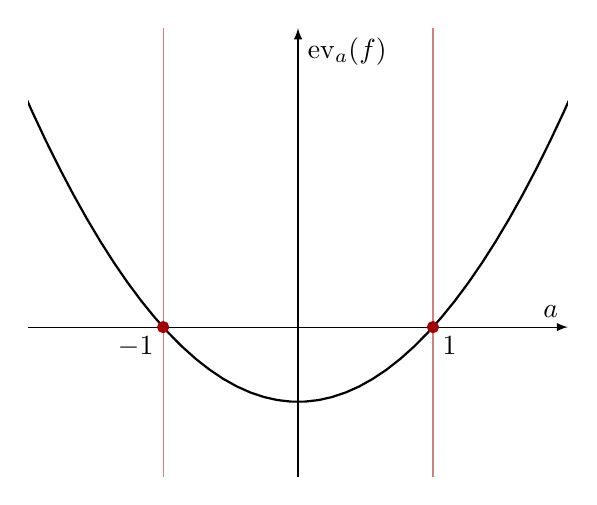
\begin{tikzpicture}
\begin{axis}[
    axis lines = middle,
    axis line style={-latex},
    xlabel = {$a$},
    ylabel = {$\ev_a(f)$},
    xmin=-2, xmax=2,
    ymin=-2, ymax=4,
    samples=100,
    xticklabels=\empty,
    yticklabels=\empty,
    ticks=none
]

% function
\addplot[thick] {x^2 - 1};

% vertical lines
\addplot[darkcandyapplered!50] coordinates {(1,-2) (1,4)};
\addplot[darkcandyapplered!50] coordinates {(-1,-2) (-1,4)};

% points
\addplot[
    only marks,
    mark=*,
    mark size=2pt,
    darkcandyapplered
] coordinates {(-1,0) (1,0)};

\node[below left] at (axis cs:-1,0) {$-1$};
\node[below right] at (axis cs:1,0) {$1$};
\end{axis}
\end{tikzpicture}
\]
όπου $f = x^2 -1 = (x-1)(x+1)\in \RR[x]$. Πώς μοιάζουν τα στοιχεία του δακτυλίου πηλίκο $\RR[x]/(x^2-1)$; 

Το $f$ έχει δύο διακεκριμένες ρίζες $\pm 1$ στο $\RR$ και κατά συνέπεια, κάθε \textquote{συνάρτηση} $g$ του $\RR[x]/(x^2-1)$ καθορίζεται από την τιμή που παίρνει όταν συναντάει τις ευθείες $y = x-1$ και $y = x+1$, δηλαδή στο ζεύγος 
\[
(\ev_{-1}(g),\ev_1(g)).
\] 
Συνεπώς, δύο \textquote{συναρτήσεις} που είναι διαφορετικές στο $\RR[x]$, αλλά παράγουν το ίδιο ζεύγος σημείων στο $\RR^2$ είναι ίδιες στον δακτύλιο πηλίκο $\RR[x]/(x^2-1)$. Για παράδειγμα, 
\[
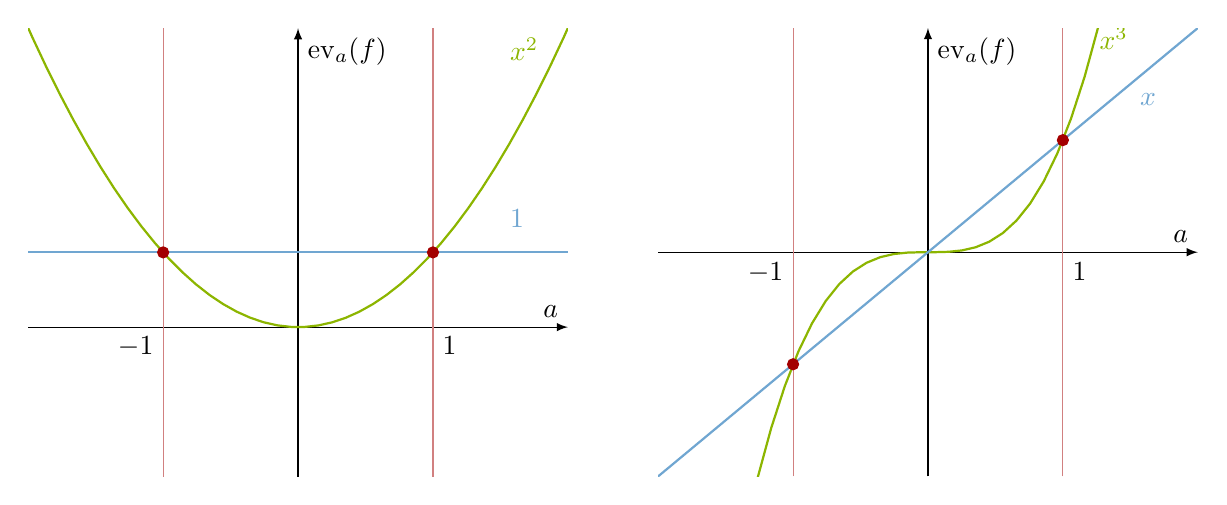
\begin{tikzpicture}
        \begin{axis}[
            axis lines = middle,
            axis line style={-latex},
            xlabel = {$a$},
            ylabel = {$\ev_a(f)$},
            xmin=-2, xmax=2,
            ymin=-2, ymax=4,
            samples=100,
            xticklabels=\empty,
            yticklabels=\empty,
            ticks=none
        ]

            % function
            \addplot[applegreen,thick] {x^2};
            \addplot[iceberg,thick] {1};

            % vertical lines
            \addplot[darkcandyapplered!50] coordinates {(1,-2) (1,4)};
            \addplot[darkcandyapplered!50] coordinates {(-1,-2) (-1,4)};

            % points
            \addplot[
                only marks,
                mark=*,
                mark size=2pt,
                darkcandyapplered
            ] coordinates {(-1,1) (1,1)};

            \node[below left] at (axis cs:-1,0) {$-1$};
            \node[below right] at (axis cs:1,0) {$1$};
            \node[below right] at (axis cs:1.5,4) {$\mathcolor{applegreen}{x^2}$};
            \node[below right] at (axis cs:1.5,1.7) {$\mathcolor{iceberg}{1}$};
        \end{axis}
    
        \begin{axis}[
            at={(8cm,0)}, 
            axis lines = middle,
            axis line style={-latex},
            xlabel = {$a$},
            ylabel = {$\ev_a(f)$},
            xmin=-2, xmax=2,
            ymin=-2, ymax=2,
            samples=100,
            xticklabels=\empty,
            yticklabels=\empty,
            ticks=none
        ]

            % function
            \addplot[applegreen,thick] {x^3};
            \addplot[iceberg,thick] {x};

            % vertical lines
            \addplot[darkcandyapplered!50] coordinates {(1,-2) (1,4)};
            \addplot[darkcandyapplered!50] coordinates {(-1,-2) (-1,4)};

            % points
            \addplot[
                only marks,
                mark=*,
                mark size=2pt,
                darkcandyapplered
            ] coordinates {(-1,-1) (1,1)};

            \node[below left] at (axis cs:-1,0) {$-1$};
            \node[below right] at (axis cs:1,0) {$1$};
            \node[below right] at (axis cs:1.2,2.1) {$\mathcolor{applegreen}{x^3}$};
            \node[below right] at (axis cs:1.5,1.5) {$\mathcolor{iceberg}{x}$};
        \end{axis}
\end{tikzpicture}
\]
όπου βλέπουμε τις ισότητες $x^2 = 1$ και $x^3 = x$ στον $\RR[x]/(x^2-1)$. Έτσι, οι πράξεις της πρόσθεσης και του πολλαπλασιασμού στο $\RR[x]/(x^2-1)$ ταυτίζονται με αυτές στο $\RR^2$ (γιατί;). Με άλλα λόγια, έχουμε τον εξής ισομορφισμό δακτυλίων
\[
\RR[x]/(x^2-1) \cong \RR[x]/(x-1) \times \RR[x]/(x+1) \cong \RR^2.
\]

Έπειτα, ας θεωρήσουμε 
\[
\begin{tikzpicture}
\begin{axis}[
    axis lines = middle,
    axis line style={-latex},
    xlabel = {$a$},
    ylabel = {$\ev_a(f)$},
    xmin=-2, xmax=2,
    ymin=-1, ymax=4,
    samples=100,
    xticklabels=\empty,
    yticklabels=\empty,
    ticks=none
]

% function
\addplot[thick] {x^2};

% vertical lines
\addplot[darkcandyapplered!50] coordinates {(0,-1) (0,4)};

% points
\addplot[
    only marks,
    mark=*,
    mark size=4pt,
    darkcandyapplered
] coordinates {(0,0)};

\node[below right] at (axis cs:0,0) {$0$};
\end{axis}
\end{tikzpicture}
\]
όπου $f = x^2 \in \RR[x]$, το οποίο έχει μία ρίζα $0$ με πολλαπλότητα δύο. Πώς μοιάζουν τα στοιχεία του δακτυλίου πηλίκο $\RR[x]/(x^2)$; 

Σκεπτόμενοι το προηγούμενο παράδειγμα, φαντάζει δελεαστικό να ταυτίσουμε τον $\RR[x]/$ $(x^2)$ με τον $\RR^2$, αλλά η δομή δακτυλίου \emph{δεν} είναι ίδια, διότι, για παράδειγμα, το στοιχείο $x^2$ είναι \emph{μηδενοδύναμο}\footnote{Ένα στοιχείο $r \in R$ ονομάζεται \defn{μηδενοδύναμο} (nilpotent) αν $r^n=0$ για κάποιο $n \ge 1$. Το να είναι ένα στοιχείο μηδενοδύναμο είναι μία \emph{αλγεβρική ιδιότητα}, δηλαδή πρέπει να διατηρείται από ισομορφιμούς (δακτυλίων).} στο $\RR[x]/(x^2)$. Η γεωμετρική ιδέα είναι ότι για να περάσουμε από το $\RR[x]$ στον δακτύλιο πηλίκο $\RR[x]/(x^2)$ δεν αρκεί να γνωρίζουμε την τιμή $a_0$ μιας \textquote{συνάρτησης} στο $0$ (τη \textquote{θέση} του), αλλά και την \textquote{κατεύθυνσή} του $a_1$: 
\[
a_0 + a_1x.
\]
Για τον λόγο αυτόν, μπορούμε να φανταστούμε το $0$ (την ρίζα πολλαπλότητας δύο του $x^2$) ως ένα \textquote{παχύ} σημείο (fat point).

Ανεξάρτητα από τη δομή δακτυλίου που έχουν τα 
\[
\RR[x]/(x^2-1), \ \RR[x]/(x^2),
\]
ως διανυσματικοί χώροι πάνω από το $\RR$ είναι ισόμορφοι.
\begin{proposition}
    \label{prop:quotient_ring_polynomials}
    Έστω $F$ ένα σώμα. Αν $f \in F[x]$ είναι ένα πολυώνυμο\footnote{Αυτά τα πολυώνυμα ονομάζονται \emph{μονικά}.} βαθμού $n$ του οποίου ο μεγιστοβάθμιος όρος είναι $1$, τότε κάθε στοιχείο του $F[x]/(f)$ μπορεί να γραφεί με μοναδικό τρόπο ως 
    \[
    a_0 + a_1\ol{x} + \cdots + a_{n-1}\ol{x^{n-1}}
    \]
    για κάποια $a_0, a_1, \dots, a_{n-1} \in F$, όπου $\ol{x^i} \coloneqq x^i + (f) \in F[x]/(f)$. Ειδικότερα, το σύνολο 
    \[
    \{1, \ol{x}, \dots, \ol{x^{n-1}}\}
    \]
    αποτελεί βάση του $F[x]/(f)$ ως $F$-διανυσματικού χώρου.
\end{proposition}
\begin{proof}[Απόδειξη]
    Ο δεύτερος ισχυρισμός είναι απλώς μια αναδιατύπωση του πρώτου (γιατί;). Για τον πρώτο, έστω $g \in F[x]$. Από το Θεώρημα 3.3 έπεται ότι 
    \[
    g = qf + \left(
        a_0 + a_1x + \cdots + a_{n-1}x^{n-1}
    \right)
    \]
    για κάποια $a_0, a_1, \dots, a_{n-1} \in F$ και $q \in F[x]$. Περνώντας στο $F[x]/(f)$ προκύπτει ότι 
    \[
    g = a_0 + a_1\ol{x} + \cdots + a_{n-1}\ol{x^{n-1}} \ \in F[x]/(f).
    \]

    Μένει να δείξουμε ότι αν
    \[
    a_0 + a_1\ol{x} + \cdots + a_{n-1}\ol{x^{n-1}} = 
    b_0 + b_1\ol{x} + \cdots + b_{n-1}\ol{x^{n-1}}
    \]
    τότε $a_i = b_i$, για κάθε $0 \le i \le n-1$, ή ισοδύναμα αν 
    \[
    c_0 + c_1\ol{x} + \cdots + c_{n-1}\ol{x^{n-1}} = 0
    \]
    στο $F[x]/(f)$, τότε \[c_0 = c_1 = \cdots = c_{n-1} = 0.\]

    Πράγματι, έστω
    \[
    \ol{g} = c_0 + c_1\ol{x} + \cdots + c_{n-1}\ol{x^{n-1}} = 0,
    \]
    στο $F[x]/(f)$, για κάποιο $g \in F[x]$. Αρκεί να δείξουμε ότι $g=0$. Επειδή $\ol{g} = 0$ έπεται ότι $g \in (f)$ και γι αυτό 
    \[
    g = qf
    \]
    για κάποιο $q \in F[x]$. Αν $g \neq 0$, τότε από την Ταυτότητα (3.1) 
    \[
    n - 1 \ge \deg(g) = \deg(q) + \deg(f) \ge \deg(f) = n
    \]
    τ' οποίο είναι αδύνατο. Άρα, $g=0$ και η απόδειξη ολοκληρώνεται.
\end{proof}

Τέλος, ας θεωρήσουμε 
\[
\begin{tikzpicture}
\begin{axis}[
    axis lines = middle,
    axis line style={-latex},
    xlabel = {$a$},
    ylabel = {$\ev_a(f)$},
    xmin=-2, xmax=2,
    ymin=-1, ymax=4,
    samples=100,
    xticklabels=\empty,
    yticklabels=\empty,
    ticks=none
]

% function
\addplot[thick] {x^2+1};
\end{axis}
\end{tikzpicture}
\]
όπου $f = x^2 +1 \in \RR[x]$, το οποίο δεν έχει καμμία ρίζα στο $\RR$. Πώς μοιάζουν τα στοιχεία του δακτυλίου πηλίκο $\RR[x]/(x^2+1)$; 

Από την Πρόταση \ref{prop:quotient_ring_polynomials} γνωρίζουμε ότι έχουν την μορφή 
\[
a + b\ol{x}
\]
για κάποια $a, b \in \RR$. Οι πράξεις της πρόσθεσης και του πολλαπλασιασμού στον δακτύλιο πηλίκο έχουν την μορφή 
\begin{align*}
    (a+b\ol{x}) + (c + d\ol{x}) &= (a+c) + (b+d)\ol{x} \\
    (a+b\ol{x})(c + d\ol{x}) &= ac + ad\ol{x} + bc\ol{x} + bd\ol{x}^2 \\
    &= (ac -bd) + (ad + bc)\ol{x}
\end{align*}
οι οποίες δεν είναι άλλες από τις αντίστοιχες πράξεις στο σώμα $\CC$ των μιγαδικών αριθμών. Με άλλα λόγια, έχουμε τον ισομορφισμό δακτυλίων 
\[
\RR[x]/(x^2+1) \cong \CC.
\]
Στην περίπτωση αυτή, παιρνώντας από το $\RR[x]$ στο $\RR[x]/(x^2+1)$, το $x$ πήρε την μορφή του φανταστικού $i$.

\begin{remark}
    Ο τελευταίος ισομορφισμός μας πληοροφρεί ότι το $\CC$ είναι το σώμα που προκύ\-πτει από το $\RR$ \textquote{προσθέτοντας} την ρίζα του πολυωνύμου $x^2+1$. Αυτό είναι ένα παράδειγμα \emph{απλής επέκτασης σωμάτων}. Για περισσότερες πληοροφορίες παραπέμπουμε στο \cite[Κεφάλαιο 13]{DF04}.
\end{remark}

Τι γίνεται στην περίπτωση που έχουμε περισσότερες από μία μεταβλητές; Για $a_1, a_2,\dots,$ $a_n \in R$, ο πυρήνας του ομομορφισμού εκτίμησης $\ev_{a_1, a_2, \dots, a_n} : R[x_1, x_2, \dots, x_n] \to R$ είναι 
\[
\ker(\ev_{a_1, a_2, \dots, a_n}) = (x_1-a_1, x_2-a_2, \dots, x_n-a_n)
\]
και γι αυτό 
\[
R[x_1, x_2, \dots, x_n] / (x_1-a_1, x_2-a_2, \dots, x_n-a_n) \cong R^n
\]
κατά αναλογία με την περίπτωση της μίας μεταβλητής. 

Επίσης, έχουμε τον ομομορφισμό δακτυλίων 
\begin{align*}
        \ev : R[x_1, x_2, \dots, x_n] &\to \fF(R^n,R) \\
                f  &\mapsto \ev_{\bullet}(f)
    \end{align*}
    όπου 
    \begin{align*}
        \ev_{\bullet}(f) : R^n &\to R \\
                           (a_1, a_2, \dots, a_n) &\mapsto \ev_{a_1, a_2, \dots, a_n}(f)
\end{align*}
ο οποίος μας επιτρέπει να φανταζόμαστε τα πολυώνυμα στις $n$ μεταβλητές ως πολυωνυμικές συναρτήσεις του $R^n$. 

Όμως, στην περίπτωση αυτή μπορεί να προκύψουν άπειρες ρίζες. Για παράδειγμα, 
\[
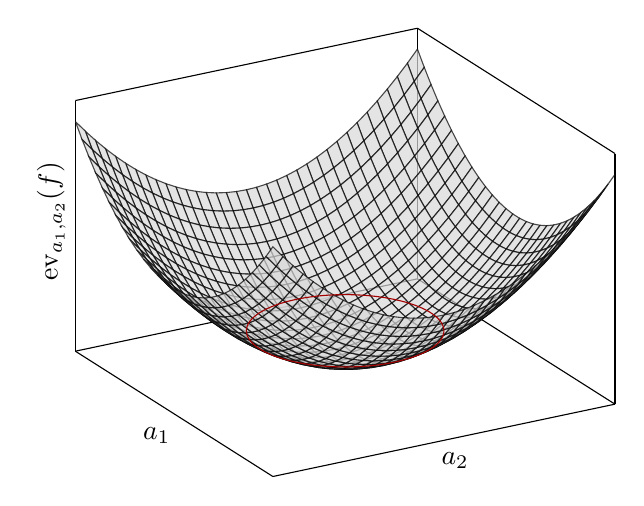
\begin{tikzpicture}
\begin{axis}[
    view={60}{30},
    xlabel={$a_1$},
    ylabel={$a_2$},
    zlabel={$\ev_{a_1,a_2}(f)$},
    domain=-2:2,
    y domain=-2:2,
    xticklabels=\empty,
    yticklabels=\empty,
    zticklabels=\empty,
    ticks=none
]

\addplot3[
    surf,
    shader=flat,
    draw=black,
    fill=gray!30,
    samples=30,
    samples y=35,
    opacity=0.7
]
{x^2 + y^2 - 1};

\addplot3[
    darkcandyapplered,
    domain=0:360,
    samples=100
]
({cos(x)}, {sin(x)}, {0});

\end{axis}
\end{tikzpicture}
\]
όπου $f = x_1^2 + x_2^2 - 1 \in \RR[x_1, x_2]$ με τις ρίζες του να \textquote{κατοικούν} στον μοναδιαίο κύκλο. Στην περίπτωση αυτή, ο δακτύλιος πηλίκο 
\[
\RR[x_1, x_2] / (x_1^2 + x_2^2 -1)
\]
έχει άπειρη διάσταση ως $\RR$-διανυσματικός χώρος με βάση 
\[
\{1, x_1, x_1^2, \dots \} \cup \{x_2, x_1x_2, x_1^2x_2, \dots\}.
\]

Έχοντας κατά νου ότι $\RR[x_1,x_2] = (\RR[x_1])[x_2]$, θα μπορούσαμε να γράψουμε 
\[
\RR[x_1, x_2] / (x_1^2 + x_2^2 -1) = 
\mathcolor{gray}{\RR[x_1]}[x_2] / ((\mathcolor{gray}{-1 + x_1^2}) + x_2^2)
\]
και να μιμηθούμε την κατασκευή της Πρότασης \ref{prop:quotient_ring_polynomials} για να γράψουμε 
\[
\RR[x_1, x_2] / (x_1^2 + x_2^2 -1) = 
\RR[x_1] \oplus \RR[x_1]x_2
\]
μετατρέποντάς το έτσι σε ένα αντικείμενο \textquote{πεπερασμένης διάστασης}. Αυτό δεν είναι πια διανυσματικός χώρος, καθώς το $\RR[x_1]$ δεν αποτελεί σώμα, αλλά ένα \emph{$\RR[x_1]$-πρότυπο}, μια δομή η οποία γενικεύει την έννοια του διανυσματικού χώρου επιτρέποντας τον βαθμωτό πολλαπλασιασμό με στοιχεία από έναν αυθαίρετο δακτύλιο. Αργότερα, θα επανέλθουμε στην οπτική του πολυωνυμικού δακτυλίου ως δακτυλίου συναρτήσεων. Στις επόμενες ενότητες θα μελετήσουμε πρότυπα πάνω από δακτυλίους.

\begin{thebibliography}{99}
    \bibitem{VDEMT13}
    Δ. Α. Βάρσος, Δ. Ι. Δεριζιώτης, Ι. Π. Εμμανουήλ, Μ. Π. Μαλιάκας και Ο. Π. Ταλέλλη, 
    \emph{Μια Εισαγωγή στην Άλγεβρα}, 
    τρίτη έκδοση, Εκδόσεις Σοφία, 2013.
    %
    \bibitem{DF04}
    D. S. Dummit και R. M. Foote, 
    \textit{Abstract algebra},
    third edition, Wiley, 2004. 
    %
    \bibitem{Mpe15}
    Α. Μπελιγιάννης, 
    \textit{Μια Εισαγωγή στη Βασική Άλγεβρα},
    Κάλλιπος, 2015. (διαθέσιμο \href{https://dx.doi.org/10.57713/kallipos-547}{εδώ})
\end{thebibliography}
\end{document}